\begin{figure}[thb]
  \centering
    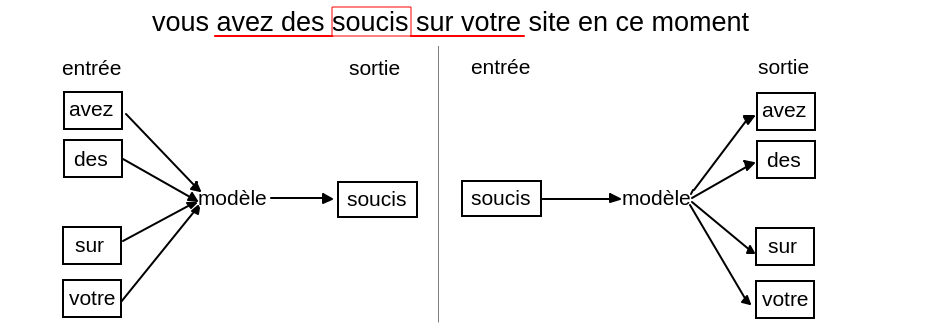
\includegraphics[width=14cm]{./Chapitre6/figures/cbow_skip.png}
    \caption{Représentation de l'apprentissage des word2vec selon deux algorithmes : le \textit{CBOW} (gauche) et le \textit{skip-gram} (droite). Ici on utilise un contexte de 5 mots, soit le mot cible entouré en rouge et deux mots de chaque coté, soulignés en rouge.
 %La partie gauche correspond à l'apprentissage avec \textit{CBOW} et la partie droite à l'apprentissage avec \textit{skip-gram}.
 }
    \label{fig:cbow_skip}
\end{figure}
